\documentclass[border=5pt]{standalone}

\usepackage[utf8]{inputenc}
\usepackage[T1]{fontenc}
\usepackage{tikz}
\usetikzlibrary{automata, positioning, arrows.meta}

\begin{document}
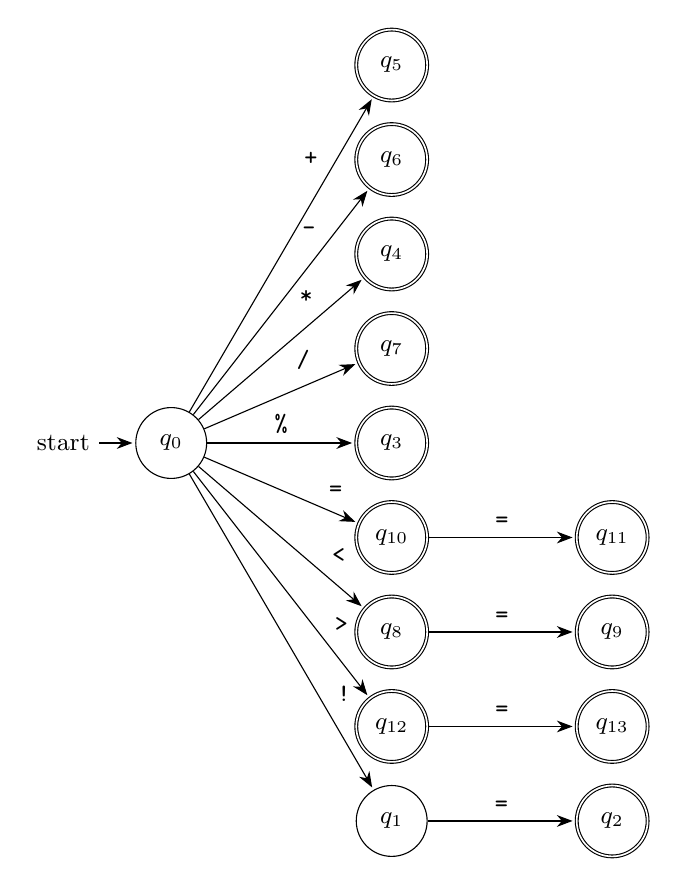
\begin{tikzpicture}[
    on grid,
    auto,
    node distance=1.2cm and 2.8cm,
    every state/.style={draw, circle, minimum size=0.9cm, inner sep=0pt,
                        font=\small},
    >={Stealth[length=2mm]},
    shorten >=1pt,
    font=\small
  ]


  \node[state, accepting]                   (mais)  {$q_5$};
  \node[state, accepting, below=of mais]    (menos) {$q_6$};
  \node[state, accepting, below=of menos]   (ast)   {$q_4$};
  \node[state, accepting, below=of ast]     (barra) {$q_7$};
  \node[state, accepting, below=of barra]   (pct)   {$q_3$};


  \node[state, accepting, below=of pct]     (igual) {$q_{10}$};
  \node[state, accepting, below=of igual]   (menor) {$q_8$};
  \node[state, accepting, below=of menor]   (maior) {$q_{12}$};

  
  \node[state, below=of maior]              (exc)   {$q_1$};


  \node[state, initial, left=of pct] (q0) {$q_0$};


  \node[state, accepting, right=of igual] (igualigual) {$q_{11}$};
  \node[state, accepting, right=of menor] (menorigual) {$q_9$};
  \node[state, accepting, right=of maior] (maiorigual) {$q_{13}$};
  \node[state, accepting, right=of exc]   (diferente)  {$q_2$};

  \path[->]
    (q0) edge node[pos=0.75] {\texttt{+}} (mais)
    (q0) edge node[pos=0.75] {\texttt{-}} (menos)
    (q0) edge node[pos=0.75] {\texttt{*}} (ast)
    (q0) edge node[pos=0.75] {\texttt{/}} (barra)
    (q0) edge node            {\texttt{\%}} (pct)
    (q0) edge node[pos=0.75] {\texttt{=}} (igual)
    (q0) edge node[pos=0.75] {\texttt{<}} (menor)
    (q0) edge node[pos=0.75] {\texttt{>}} (maior)
    (q0) edge node[pos=0.75] {\texttt{!}} (exc)

    (igual) edge node {\texttt{=}} (igualigual)
    (menor) edge node {\texttt{=}} (menorigual)
    (maior) edge node {\texttt{=}} (maiorigual)
    (exc)   edge node {\texttt{=}} (diferente);

\end{tikzpicture}
\end{document}